\documentclass[conference]{IEEEtran}
\IEEEoverridecommandlockouts
%Template version as of 6/27/2024

\usepackage{cite}
\usepackage{amsmath,amssymb,amsfonts}
\usepackage{algorithmic}
\usepackage{graphicx}
\usepackage{textcomp}
\usepackage{xcolor}
\usepackage{tikz}
\usepackage{orcidlink}
\hypersetup{
    colorlinks=false,
    pdfborder={0 0 0},
}

\newcommand{\TODO}[1]{\textbf{\textcolor{red}{TODO: #1}}}

\def\BibTeX{{\rm B\kern-.05em{\sc i\kern-.025em b}\kern-.08em
    T\kern-.1667em\lower.7ex\hbox{E}\kern-.125emX}}

\begin{document}

\title{
    Investigating Protein Folding Dynamics Using Molecular Dynamics Simulations-based Approaches
}

\author{\IEEEauthorblockN{Christian Nix\,\orcidlink{0009-0006-5718-3452}}
\IEEEauthorblockA{\textit{School of Computation, Information and Technology (CIT)} \\
\textit{Technical University of Munich}\\
Munich, Germany \\
christian.nix@tum.de}
}

\maketitle

\begin{abstract}
\TODO{Lorem ipsum dolor sit amet, consetetur sadipscing elitr, sed diam nonumy eirmod tempor invidunt ut labore et dolore magna aliquyam erat, sed diam voluptua. At vero eos et accusam et justo duo dolores et ea rebum. Stet clita kasd gubergren, no sea takimata sanctus est Lorem ipsum dolor sit amet. Lorem ipsum dolor sit amet, consetetur sadipscing elitr, sed diam nonumy eirmod tempor invidunt ut labore et dolore magna aliquyam erat, sed diam voluptua. At vero eos et accusam et justo duo dolores et ea rebum. Stet clita kasd gubergren, no sea takimata sanctus est Lorem ipsum dolor sit amet. Lorem ipsum dolor sit amet, consetetur sadipscing elitr, sed diam nonumy eirmod tempor invidunt ut labore et dolore magna aliquyam erat, sed diam voluptua. At vero eos et accusam et justo duo dolores et ea rebum. Stet clita kasd gubergren, no sea takimata sanctus est Lorem ipsum dolor sit amet. Duis autem vel eum iriure dolor in hendrerit in vulputate velit esse molestie consequat, vel illum dolore eu feugiat nulla facilisis at vero eros et accumsan et iusto odio dignissim qui blandit praesent luptatum zzril delenit augue duis dolore te feugait nulla facilisi.}
\end{abstract}

\begin{IEEEkeywords}
\TODO{Index words to be added in the end.}
\end{IEEEkeywords}

\section{Introduction}
Proteins are fundamental in driving biological processes and form the basic building blocks that life relies on \cite{eisenberg2000protein}. They are pivotal in almost all cellular processes, thus motivating their study in fields such as medicine, chemistry, or biophysics. Proteins play essential roles in regulation, transportation, signaling, immune responses, and metabolism, among others. \cite[pp.~163ff., pp.~225ff.]{buxbaum2007fundamentals} Chemically, proteins are a polymer of 20 canonical amino acids that have unique side-chains giving them unique chemical properties, such as hydrophobicity, charge, or polarity. Neighboring amino acids are linked via peptide bonds formed between their \textit{amino} and carboxyl (\textit{acid}) groups, thus forming the protein's backbone from which their distinct side-chains extend. \cite{stollar2020uncovering}

Protein structure is commonly described as four hierarchical levels: primary, secondary, tertiary, and quaternary structure. The \textit{primary structure} refers to the linear sequence of amino acids in the protein chain. Given the chemical properties of neighboring amino acids, \textit{secondary structure} elements, such as $\alpha$-helices or $\beta$-sheets, can be formed. The secondary structure is stabilized by hydrogen bonds between backbone atoms. The \textit{tertiary structure} describes the overall 3D arrangement of the protein chain, including the side-chains, i.e., the determination of all atoms in 3D space. The tertiary structure is stabilized by a broad set of interactions, such as van der Waals forces, hydrogen bonds, ionic interactions, and disulfide bridges. Finally, some proteins consist of multiple polypeptide chains (i.e., multiple protein subunits), whose arrangement is described by the \textit{quaternary structure}. \cite[pp.~65ff.]{kessel2018introduction}

Generally speaking, protein function, and thus the protein's biochemical role, is determined by its 3D structure, motivating the study of protein structures and how proteins assume these structures \cite{lee2007predicting}. However, proteins are not static entities, but rather dynamic molecules that can undergo conformational changes to perform their functions. Therefore, understanding protein dynamics is crucial for a comprehensive understanding of protein function. \cite{teilum2009functional} Additionally, misfolded proteins can lead to various diseases, such as Alzheimer's, Parkinson's, or cystic fibrosis, further highlighting the importance of understanding protein folding as a dynamic process \cite{valastyan2014mechanisms}.

\subsection{Protein Folding and its Importance}
So far, we have established that knowing the 3D structure of proteins is important for understanding their function and role in biological processes. However, the process of protein folding itself is highly complex and not yet fully understood \cite{tsuboyama2023mega}. Anfinsen's Nobel prize-winning work demonstrated that the primary structure (i.e., the amino acid sequence) of a protein determines its final 3D structure, implying that all information necessary for folding is self-contained \cite{anfinsen1973principles}. However, if a protein were to randomly sample all possible conformations its primary sequence could take, the time required to fold would be much beyond the biologically relevant timescales (milliseconds to seconds) observed in nature \cite{levinthal1969fold, dobson2003protein}. For example, assuming 10 possible configurations per amino acid residue, a small protein of 100 residues would have $10^{100}$ possible conformations. A rotation around a single bond takes roughly $10^{-12}$ s \cite{lee2025ultrafast}, leading to a total time of $10^{88}$ s or roughly $10^{80}$ years to sample all conformations. This discrepancy is known as Levinthal's paradox \cite{levinthal1969fold}. Since we know that proteins do fold on biologically relevant timescales, there must be some guiding principles that direct the folding process efficiently.

To describe the folding process and its driving forces, we make use of the Gibbs free energy $G = H - TS$, where $H$ is the enthalpy, $T$ the temperature, and $S$ the entropy \cite[pp.~76ff.]{AtkinsDePaula2006}. The Gibbs energy is valid, because folding occurs at constant pressure and temperature \cite{ghelis2012protein, pain2000mechanisms, bryngelson1995funnels}. As becomes apparent from the definition of $G$, folding is driven by enthalpic ($H$) and entropic contributions ($TS$). For example, a main driver of folding is the hydrophobic effect, where non-polar residues cluster together \cite{durell2017hydrophobic}. This benefits the enthalpy via van der Waals forces between the residues, but also increases the entropy by releasing ordered water molecules into the bulk solvent \cite[pp.~280ff.]{KlostermeierRudolph2024}. If we now consider the free energy as a function of the protein's conformation, we arrive at the concept of the energy landscape of protein folding. In Levinthal's paradox, the energy landscape was assumed to be flat, with only the native, folded state being energetically favorable, resulting in random searching. During the 1990s, the concept of the energy landscape as a folding funnel was introduced (Figure \ref{fig:intro:funnel}). \cite{bryngelson1995funnels, onuchic1997theory}

\begin{figure}[b]
    \centering
    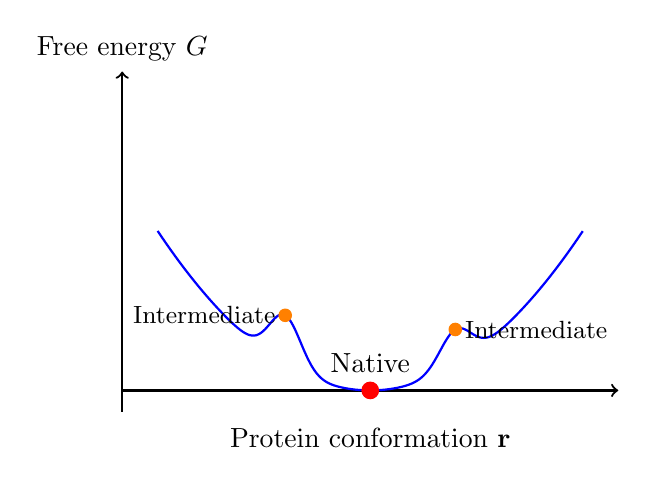
\begin{tikzpicture}[scale=1.5]
  % Define scaling factors
  \def\xscale{0.6}
  \def\yscale{0.6}
  
  % Function: f(x) = 0.25*x^2 + 0.7*exp(-10*(x+1.2)^2) + 0.5*exp(-10*(x-1.2)^2)
  % This creates a quadratic well with two local minima (intermediates)
  
  % Draw axes
  \draw[->, thick] (-3.5*\xscale,0) -- (3.5*\xscale,0) node[right] {};
  \draw[->, thick] (-3.5*\xscale,-0.3*\yscale) -- (-3.5*\xscale,4.5*\yscale) node[above] {Free energy $G$};
  
  % Plot the energy landscape
  \draw[thick, blue, smooth] plot[domain=-3:3, samples=100] 
    ({(\x)*\xscale}, {(0.25*\x*\x + 0.7*exp(-10*(\x+1.2)*(\x+1.2)) + 0.5*exp(-10*(\x-1.2)*(\x-1.2)))*\yscale});
  
  % Mark the native state (global minimum at x=0)
  \filldraw[red] (0,0) circle (2pt);
  \node[above=3pt] at (0,0) {Native};
  \node[below=10pt] at (0,0) {Protein conformation $\mathbf{r}$};
  
  % Mark intermediate states (local minima at x ≈ ±1.2)
  \filldraw[orange] ({-1.2*\xscale},{(0.25*1.44 + 0.7)*\yscale}) circle (1.5pt);
  \node[left, font=\small] at ({-1.2*\xscale},{(0.25*1.44 + 0.7)*\yscale}) {Intermediate};
  
  \filldraw[orange] ({1.2*\xscale},{(0.25*1.44 + 0.5)*\yscale}) circle (1.5pt);
  \node[right, font=\small] at ({1.2*\xscale},{(0.25*1.44 + 0.5)*\yscale}) {Intermediate};
  
\end{tikzpicture}
    \caption{\TODO{Temporary Fig} Schematic representation of a high-dimensional protein folding funnel which is a free energy function $G$ of protein conformation $\mathbf{r}$. The native state corresponds to the global minimum of the free energy. Local minima represent meta-stable folding intermediates which originate from conformational changes. Kinetic conversion between minima requires overcoming energy barriers and can thus be slow.}
    \label{fig:intro:funnel}
\end{figure}

As can be seen in Figure \ref{fig:intro:funnel}, the folding funnel concept correctly captures that conformations along a folding pathway do not have the same energy. The idealized funnel shape arises from the assumption that each newly formed native contact (i.e., a contact that exists in the native structure) lowers the free energy, leading to a monotonic decrease in free energy as folding progresses. \cite[pp.~283ff.]{KlostermeierRudolph2024} However, the energy landscape is much more rugged in reality, with many local extrema. For example, conformations stemming from rotating a side-chain may differ by small differences in energy, thus these conformations are interconverted rapidly. On the other hand, larger conformational changes, such as forming or breaking tertiary structure elements, may lead to greater energy changes and therefore result in local minima that are harder to escape from. \cite{bryngelson1995funnels} These local minima, given sufficiently large energy barriers, can lead to meta-stable states and folding intermediates \cite{dill2008protein}.

The protein folding problem is not limited to predicting the final folded structure, but is also interested in understanding the folding pathways, i.e., the process by which a protein transitions from its unfolded to folded state through these various intermediates and meta-stable states \cite{eaton2000fast}. Ground-breaking methods such as AlphaFold \cite{senior2020improvedAF1, jumper2021highlyAF2, abramson2024accurateAF3} have essentially solved the prediction of the final folded structure, although they do not reveal \emph{how} proteins reach that state \cite{outeiral2022current}. Importantly, proteins do not necessarily fold via a single, well-defined pathway, but can utilize multiple pathways to reach the native state \cite{sridevi2004increasing}. As a result, we must identify not only the final native state, but also the various folding intermediates along the pathways and determine the kinetics of folding, i.e., the rates at which transitions between conformational states occur, especially those that are rate-limiting and therefore control the overall folding speed \cite{gelman2014fast}.

\subsection{Studying Protein Folding Dynamics}
\label{sec:intro:studying_folding}
Until the 1990s, protein folding dynamics were primarily studied experimentally using \textit{stopped-flow} techniques, which allowed a temporal resolution of around 1 ms \cite{gibson19696}. At the same time, atomistic molecular dynamics (MD) simulations were limited to nanosecond timescales. As a result, all (at the time) described protein folding events occurred on timescales inaccessible to MD simulations. \cite{eaton2021modern} However, the development of laser-based temperature-jump (T-jump) techniques enabled the experimental study of protein folding on nanosecond timescales \cite{phillips1995ultrafast}. Nonetheless, T-jump experiments cannot provide information about the underlying conformational rearrangements as they report only global relaxation kinetics \cite{eaton2021modern}. In contrast, experimental methods such as Förster resonance energy transfer (FRET) can yield insights into the distances between specific residues, thus providing some structural information \cite{schuler2008protein}. However, experimental methods are generally limited in the level of detail they can provide about the folding process, motivating the use of MD simulations to allow atomistic insights into folding dynamics \cite{piana2014assessing}.

In molecular dynamics, the motion of atoms is propagated using classical mechanics, by integrating, e.g., Newton’s equations of motion \cite[pp.~358ff.]{santamaria2023molecular}. The forces acting on the atoms are typically obtained from a molecular mechanics force field\footnote{Since MD simulations are fully controlled by the user, the forces acting on the system do not have to correspond strictly to physical reality but can also be altered, e.g., by mixing classical mechanics with quantum mechanical effects \cite{warshel1976theoretical}.}, which provides an approximate potential energy function \cite[pp.~298ff.]{santamaria2023molecular}. As a result, running MD simulations allows us to explore the conformational space according to the Boltzmann distribution (given some assumptions, which we will discuss later), which includes folding events \cite{henin2022enhanced}. However, the exploration of conformational space is still stochastic, requiring us to run simulations for long enough. With increasing computational power \cite{salomon2013routine}, the use of specialized hardware \cite{shaw2008anton}, or highly parallelized simulations \cite{shirts2000screen}, MD simulations can access increasingly long timescales. \cite{hollingsworth2018molecular} Alternatively, enhanced sampling methods such as metadynamics \cite{laio2002escaping} or umbrella sampling \cite{torrie1977nonphysical} can be used to accelerate the exploration of rare conformations by biasing the sampling process, e.g., by adding biasing potential that guides the system over energy barriers \cite{henin2022enhanced}. However, since these methods bias the simulation, the downstream analysis of the resulting trajectories must be adapted accordingly \cite{kamenik2022enhanced}.

To extract meaningful insights from MD simulations, their trajectories must be analyzed appropriately. Some properties, such as the temperature, pressure, or distances, can be computed directly from (averages over) the frames of the trajectory. However, many properties of interest, such as free energies which determine folding pathways and their kinetics, depend not on the frames directly, but rather on the distribution of conformations they represent, i.e., the accessible conformational space. \cite[pp.~167ff.]{frenkel2002understanding} Analyzing the conformational space is non-trivial due its high dimensionality (e.g., three special coordinates per atom). To enable interpretation, we can project the high-dimensional conformational space onto fewer collective variables (CVs), along which we, for example, can compute free energy surfaces (FES). \cite{fiorin2013using} Collective Variables are detailed in Section \TODO{Ref}. For extracting long-timescale kinetics, a probabilistic framework such as Markov State Models (MSMs) can be applied \cite{malmstrom2014application}. These will be discussed in detail in Section \TODO{Ref}. MSMs discretize the conformational space into distinct states, enabling the quantitative prediction of transition rates and folding pathways \cite{chodera2014markov}.

\subsection{Transfer Operator Formalism}
% - Explain all the math necessary for the TICA and MSM formalism via the transfer operator

At the end of the 1990s, the transfer operator formalism was introduced to model the dynamics of molecular systems in the context of MD simulations and thus provided a principled mathematical framework for describing MD simulations \cite{schutte2001transfer}. In this section, we summarize the key concepts of this formalism that are necessary to understand the following sections on collective variables (Section \TODO{Ref}) and Markov State Models (Section \TODO{Ref}). The notation and terminology used here follow those in \cite{prinz2011markov, perez2013identification, noe2017collective}. For more detailed explanations and in depth derivations, the reader is referred to those references.

The possible conformations of a molecular system, in our case a (solvated) protein, span a high-dimensional state space $\Omega \subseteq \mathbb{R}^{3n}$, where $n$ is the number of atoms in the system. In some cases, the state space may be expanded to represent the full phase space by including momenta (then $\Omega \subseteq \mathbb{R}^{6n}$), but we will focus on the configuration space here. A trajectory generated by an MD simulation can be seen as a time series of points in this state space $\mathbf{x}(t) = \mathbf{x} \in \Omega$, i.e., the conformation of the system at time $t$. The dynamical process $\mathbf{x}(t)$ can be either time continuous or discrete. Since we are concerned with MD simulations, we will consider discrete time points $t = k \delta$, where $k \in \mathbb{N}_0$ and $\delta$ is the integration time step between frames. However, the transfer operator formalism will increasingly move away from individual trajectories or conformations and instead focus on probability distributions over the state space $\Omega$ at time $t$, denoted as $p_t(\mathbf{x}): \Omega \rightarrow \mathbb{R}_{0+}$. These probability distributions describe how likely the system is to occupy different regions of the state space at a given time $t$ and thus provide a statistical description of the ensemble that the MD simulation sampled from. We must impose some assumptions on the dynamical process $\mathbf{x}(t)$ to make the following formalism mathematically founded.

First, we assume that the process is \textit{Markovian} in $\Omega$. This means that the future state of the system $\mathbf{x}(t + \Delta t)$ depends only on its current state $\mathbf{x}(t)$. We can therefore define the transition probability density as:

\begin{equation}
    p(\mathbf{x}, \mathbf{y}; \tau) d\mathbf{y} = \mathbb{P}\left[\mathbf{x}(t + \tau) = \mathbf{y} + d\mathbf{y} | \mathbf{x}(t) = \mathbf{x}\right]
\end{equation}
$p(\mathbf{x}, \mathbf{y}; \tau)$ describes the probability density of transitioning from state $\mathbf{x}$ at time $t$ to state $\mathbf{y}$ at time $t + \tau$ (note that we require $d\mathbf{y}$ since the state space is continuous and we must integrate to get probabilities). As before, we will consider discrete time points, i.e., $\tau = m \delta$ for $m \in \mathbb{N}_0$. Similarly, we can define the transition probability from a state $\mathbf{x}$ at time $t$ to a set of states $A \subset \Omega$ at time $t + \tau$ as $p(\mathbf{x}, A; \tau) = \mathbb{P}\left[\mathbf{x}(t + \tau) \in A | \mathbf{x}(t) = \mathbf{x}\right]$.

Second, we assume that the process is (sufficiently) \textit{ergodic}, meaning that all states in $\Omega$ can be reached from any other state, such that a unique stationary distribution $\mu(\mathbf{x})$ exists. The stationary distribution can be seen as the fraction of time the system spends in different regions of the state space when the simulation time approaches infinity. As mentioned in Section \ref{sec:intro:studying_folding}, the stationary distribution for molecular dynamics simulations at constant temperature is given by the Boltzmann distribution:

\begin{equation}
    \mu(\mathbf{x}) = Z^{-1} e^{-\beta H(\mathbf{x})}
\end{equation}
where $Z$ is the partition function (normalization constant), $\beta = (k_B T)^{-1}$ is the inverse temperature with Boltzmann constant $k_B$ and temperature $T$, and $H(\mathbf{x})$ is the Hamiltonian of the system at conformation $\mathbf{x}$ (total energy).

Lastly, we assume that the process is \textit{reversible}. Thus, the transition probability satisfies the condition of detailed balance, i.e., when at equilibrium (the stationary distribution $\mu(\mathbf{x})$), the transition rate from state $\mathbf{x}$ to $\mathbf{y}$ is equal to the reverse direction: $\mu(\mathbf{x}) p(\mathbf{x}, \mathbf{y}; \tau) = \mu(\mathbf{y}) p(\mathbf{y}, \mathbf{x}; \tau)$. The condition of detailed balance is not necessary for, e.g., Markov State Models (Section \TODO{Ref}), but it simplifies the mathematical treatment so that we will assume it here. Generally, it is assumed that equilibrium MD simulations fulfill this condition \cite{prinz2011markov}.

Given these assumptions, we now focus on the change of the probability distribution $p_t(\mathbf{x})$ (different from $\mu(\mathbf{x})$) as the MD simulation progresses. If the system is at distribution $p_t(\mathbf{x})$ at time $t$, the distribution after lag-time $\tau$ will have changed (slowly approaching $\mu(\mathbf{x})$) since the system has evolved according to the transition probabilities $p(\mathbf{x}, \mathbf{y}; \tau)$ defined above. Mathematically, we can describe this change using the \textit{propagator operator} $\mathcal{P}(\tau)$, which advances the distribution $p_t(\mathbf{x})$ by lag-time $\tau$ to $p_{t + \tau}(\mathbf{y})$:

\begin{equation}
    p_{t + \tau}(\mathbf{y}) = \mathcal{P}(\tau) p_t(\mathbf{y}) = \int_{\mathbf{x} \in \Omega} p(\mathbf{x}, \mathbf{y}; \tau) p_t(\mathbf{x}) d\mathbf{x}
\end{equation}
If we now consider not the probability distribution $p_t(\mathbf{x})$ directly, but rather its relative distribution with respect to the stationary distribution $\mu(\mathbf{x})$, we can define the equivalent \textit{transfer operator} $\mathcal{T}(\tau)$ as:

\begin{align}
    u_{t + \tau}(\mathbf{y}) = \mathcal{T}(\tau) u_t(\mathbf{y}) &= \frac{1}{\mu(\mathbf{y})} \int_{\mathbf{x} \in \Omega} p(\mathbf{x}, \mathbf{y}; \tau) \mu(\mathbf{x}) u_t(\mathbf{x}) d\mathbf{x} \\
    p_t(\mathbf{x}) &= \mu(\mathbf{x}) u_t(\mathbf{x})
\end{align}
Because both operators $\mathcal{P}(\tau)$ and $\mathcal{T}(\tau)$ fulfill the Chapman-Kolmogorov equation, they can be applied arbitrarily often to propagate the distribution over multiple lag-times $\tau$.

% The key understanding is now that the eigenvalues and eigenfunctions have meaning
% We ask the reader to think about what happens if we apply the propagator operator on the stationary distribution mu(x) 
% We can understand the eigenfunctions as those distributions that remain unchanged if propagated
% In our case of molecular dynamics, these are the slowest processes of the system, which includes folding!
% The corresponding eigenvalues tell us how fast these processes are (timescales) and they follow the relation XYZ
% Thus we are interested in approximating these eigenvalues and eigenfunctions from MD data, which we will do in the following sections ref to TICA and MSMs

% Then the last bit of formalism ...

\subsection{Aim and Scope}
% - Aim of this work:
%   - Literature review and light practical work on how to investigate protein folding dynamics using MD simulations-based approaches
%   - Scope of this work:
%       - Overview over how to study the folding process in terms of the free energy surface via collective variables (historic, and SOTA models, etc.)
%       - Using Markov State Models (MSMs) to model folding kinetics and pathways (which in turn are the basis for retrieving pathways, intermediates, etc.) 
%   - Applying the above to a model protein system to demonstrate the approaches and HOPEFULLY do some minor "novel" thing (i.e. change some parameters and see what result changes etc.) in this seminar paper for my University course

\section{Collective Variables and Free Energy Surfaces}
% - Collective variables (CVs) and free energy surfaces (FES):
%   - What are CVs
%   - Why get them:
%       - Allow to visualize high-dimensional free energy landscape in low dimensions --> interpretable, intuitive, etc.
%       - Basis for enhanced sampling methods (e.g. metadynamics)
%       - By biasing MDs along CVs, we can sample rare events (e.g. folding) more efficiently, accessing relevant conformations faster
%   ==> Thus CVs are an essential backbone for studying protein folding dynamics via MD simulations

%   - But what can CVs pratcically not solve: If we want deep insights, the projection onto low-dimensional CVs can lead to loss of important information (histeric problem in MD analysis, i.e., hiding important states/transitions). But also enhanced sampling methods are not the ultimate solution for deep insights and e.g. pathway identification including kinetics and rate constants
% Kind of first work with TICAs on MD simulations: https://doi.org/10.1063/1.3554380 (2011) --> They seem to be some of the first to apply TICA to MD simulations
% Here they show that TICA == specifica version of variational approach https://doi.org/10.1063/1.4811489 (2013)
% Why TICA in the first place and genrally avout collection variables: https://doi.org/10.1016/j.sbi.2017.02.006 
% https://arxiv.org/pdf/2202.04164 --> general stuff about CVs too (but in context of enhanced sampling)
% fiorin2013using --> Using collective variables to drive MD simulations (review paper, nice)

% Free-Energy Landscape for ß Hairpin Folding from Combined Parallel Tempering and Metadynamics | Giovanni Bussi,* Francesco Luigi Gervasio,* Alessandro Laio,† and Michele Parrinello ==> CVs are used to drive metadynamics simulations but they have problems if they hide slow degrees of freedom, so they try to fix that by merging parallel tempering
% CVs go back FAR: Statistical mechanics of isomerization dynamics in liquids and the transition state approximation | Chandler 1978, isomerization but they do their math along a reaction coordinate q
% ML CVs: https://arxiv.org/pdf/2107.03943 (2021) --> Also very interesting, they mention many works. ==> Importantly, CVs need to be classified into whether they are applied after the simulation (i.e., for analysis, visualization, etc.) or during the simulation (i.e., for enhanced sampling)
% Review on CVs: Collective variables for the study of long-time kinetics from molecular trajectories: Theory and methods | Frank Noé --> rather "new" (2017)
% --> They find that a variational approach to solve the eifenvalue problem of the transfer operator is a more general form compared to how it is done in MSMs or TICA (not meaning that they become obsolete, but that they are special cases of this more general approach)
% Book on ICA (and AMUSE pp 341ff): Independent Component Analysis, Aapo Hyvarinen, Juha Karhunen, and Erkki Oja, 2001, https://www.cs.helsinki.fi/u/ahyvarin/papers/bookfinal_ICA.pdf

\section{Markov State Models and Protein Folding Kinetics}
% - Talk about what MSMs are, why people first started using them for protein folding (intuition), and then talk about the formalism in transfer operator language
% chodera2014markov --> 2014 review paper on MSMs for biomolecular dynamics

% Potential Projects
% file:///Users/christianmacbook/Downloads/978-3-540-38448-9.pdf --> Chapter 8 talks about some math for MD that needs to be assumed (pdf page 293)
% ------------
% - A general concern with TICA and the variational approach is computational efficiency for large systems and long trajectories. The computational effort scales with N^2 for N input coordinates, which becomes intractable if huge basis sets are used, such as the set of distances between all residues or atoms of a protein. The recently proposed hierarchical TICA method can obtain a coarse-grained yet accurate solution of the full TICA problem more efficiently [60], but there is still room for improvements in this area. (from Noe review)
%==> In https://doi.org/10.1063/1.4811489: It is shown that the scalar product of the eigenfunctions (which are the linear combinations of input order parameters) approximates the relaxation timescale from below. If we simply maximize this quantity via gradient ascent, we can obtain the linear coefficients for the eigenfunctions without computing the covariance matrices (in turn avoiding the N^2 scaling, but we need an iterative method). But from what I am just reading, it may be that the approximation is only valid for the slowest timescale (first non-trivial eigenfunction)
%--------------
% - Or what if we apply the formalism found here to the problem of training NNs. From ChatGPT: Use stochastic gradient MCMC (SGLD / SGHMC) to sample: If you want a stationary distribution 𝑝 ( 𝜃 ) ∝ 𝑒 − 𝛽 𝐿 ( 𝜃 ) p(θ)∝e −βL(θ) over parameters, use SGLD: these add calibrated Gaussian noise to gradient updates and have a known stationary distribution (under assumptions). They are exactly the analogue of Langevin / Hamiltonian dynamics in parameter space. Classic refs: Welling & Teh (SGLD) and SGHMC work. (maybe this is (koopman training) related: https://arxiv.org/pdf/2006.02361) IMPORTANT for applying TICA: "We also assume that the dynamics are statistically reversible, i.e., that the molecular system is simulated in thermal equilibrium." from https://doi.org/10.1063/1.4811489 --> Check if this is given

\section*{Acknowledgment}

\TODO{Acknowledgments to be added in the end.}

\bibliographystyle{IEEEtran}
\bibliography{references}

\end{document}
